\chapter{Unión de imágenes}
\label{capitulo5}
\lhead{Capítulo 5. \emph{Unión de imágenes}}


\section{Introducción}
El objetivo final de la creación de un mosaico, es lograr un mapa que represente de la mejor forma la trayectoria recorrida. Esto es, que sea visualmente congruente y que no presente ningún tipo de discontinuidades de modo que todo parezca una misma imagen. De las primeras etapas se manifiestan muchos errores producto de los problemas ya planteados, si bien a lo largo del proceso éstos se intentan reducir lo mas posible, siempre es necesaria la etapa final de fusión para lograr los objetivos propuestos.

En esta sección se describen los algoritmos utilizados para lograr fusionar las imágenes del mosaico, como ya se especificó fueron seleccionados aquellos que presentaron resultados importantes en diversos estudios externos, y se implementaron en conjunto para lograr resultados mucho mas robustos. Estos se detallan a continuación en el orden de aplicación sobre el mosaico: linea de corte, ajuste de color y finalmente la fusión ponderada.

Finalmente se muestran los resultados con su respectivo análisis de aplicar cada uno de los algoritmos aquí descritos.
\clearpage


\section{Linea de costura}
Este algoritmo es aplicado en primer lugar, ya que el resto de métodos requieren conocer de antemano los límites de cada imagen. 
A diferencia de los anteriores, este tipo de algoritmos es el único que toma en cuenta la información que comparten las imágenes en el área que tienen en común, con lo cual su implementación logra corregir la mayor cantidad de imperfecciones. 


\subsection{Corte por grafo}

Este es un método derivado de la teoría de grafos, donde la idea es separar un grafo con conexiones simples en dos grafos separados con un mínimo costo de separación. Se define un grafo $\mathcal{G} = \langle \mathcal{N}, \mathcal{E} \rangle$ como un conjunto de nodos $\mathcal{N}$, conectados por enlaces $\mathcal{E}$. Cada enlace conecta dos nodos y tiene asociado un costo o peso $\mathcal{W}(p, q) \,\, p,q \in \mathcal{N}$ --- cuando se habla de conexión simple, se refiere a que el costo en los enlaces está asociado para ambas direcciones $\mathcal{W}(p, q) = \mathcal{W}(p, q)$ ---. Se dice que dos grafos están separados si no se tiene ningún enlace que conecte dos nodos entre los grafos. Definimos $\mathcal{S}$ y $\mathcal{T}$ como los grafos separados que se tienen luego de aplicar el corte en $\mathcal{G}$. El método para determinar el mejor corte se basa en encontrar el camino entre los enlaces que logra separa un grafo en dos, con el mínimo costo de corte, donde el costo del corte es la suma de los pesos de todos los enlaces del camino seleccionado.

En el conjunto de nodos en el grafo se cuentan con dos especiales o nodos terminales, el inicio ($\mathtt{I}$) y el final ($\mathtt{F}$), donde el resto de píxeles en la imagen corresponden con un nodo no terminal. En aplicaciones de visión por computadora, cuando se desea unir dos imágenes en una región de intersección, lo que se busca es lograr un etiquetado de píxeles que permita distinguir que nodos corresponden a cada imagen en el área de intersección.

Se presenta en la ecuación \ref{funcion-corte} la función de coste que etiqueta los nodos, y minimiza el costo del corte.
\begin{equation}
C(f) = \sum_{_p\in \mathcal{N}}^{} D_p(f_p) + \sum_{_p,_q \in \mathcal{N} - \{\mathtt{I},\mathtt{F}\}}^{} \mathcal{W}_p,_q (f_p, f_q)
\label{funcion-corte}
\end{equation}
Donde $p$ es un nodo que pertenece al conjunto de nodos no terminales $\mathcal{N} - \{\mathtt{I},\mathtt{F}\}$. El término $D_p(f_p)$ es el costo de asignar una etiqueta $f_p$ ($f_p \in \{0,\,1\}$) al nodo $p$ --- en este caso una etiqueta binaria, asociando el píxel a una imagen u otra ---. El término $\mathcal{W}_p,_q (f_p, f_q)$ es el costo de asociar una etiqueta al nodo $_p$ y una distinta al nodo $_q$.

Una gran diferencia de intensidades entre píxeles adyacentes representa un fuerte indicador de la existencia de un borde o contorno entre dos objetos, es decir, que el costo de un enlace se puede definir como el inverso de la diferencia entre la intensidad de los píxeles que conecta. Siendo $I(p)$ la intensidad de un píxel $p$, se defina el coso de cada enlace como:
\begin{equation}
\mathcal{W}_p,_q = 255 - |I(p) - I (q)|
\label{costo-corte}
\end{equation}
Si bien se consideran los parámetros necesarios con esa función, se obtienen resultados mucho mas robustos usando una función exponencial \cite{graph-opencv}:
\begin{equation}
\mathcal{W}_p,_q = e^{\left(\frac{255-|I(p) - I (q)|}{2 \sigma}  \right) }
\label{costo-corte}
\end{equation}
Donde $\sigma$ es la desviación estándar de la imagen, y siendo válido para los casos en los que $f_p \neq f_q$, indicando que ambos nodos pertenecen serán separados por la linea de corte.

\begin{figure}[h]
	\centering
	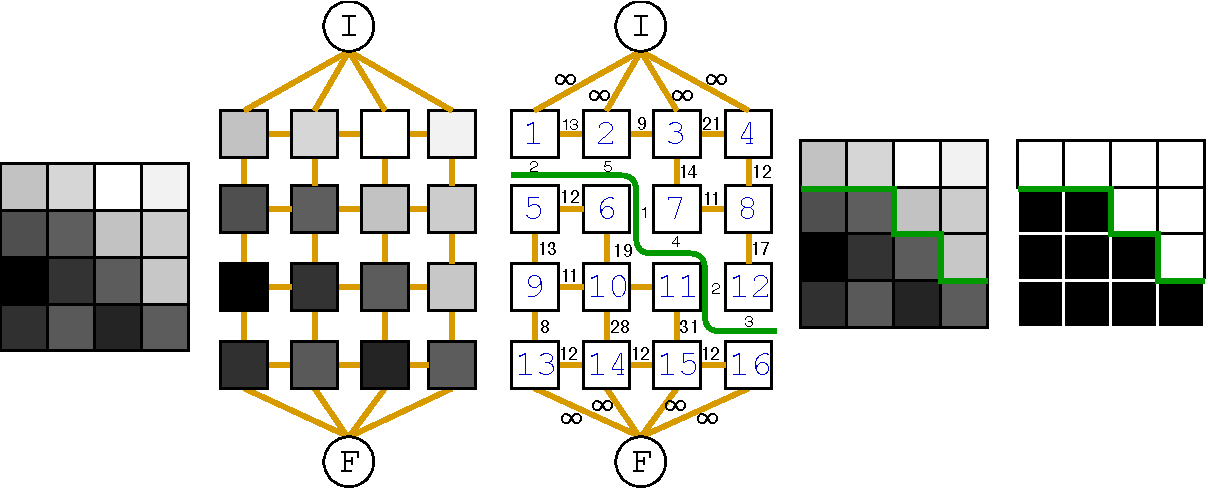
\includegraphics[width=1\linewidth]{grafo-completo.pdf}
	\caption[Corte por grafo]{De izquierda a derecha: imagen original, creación de nodos y enlaces, se asignan los pesos y se halla la linea de corte, finalmente se binariza la imagen según las etiquetas para crear una mascara.}
	\label{imagen:grafo}
\end{figure}
Refiriéndonos a la figura \ref{imagen:grafo}, se observa el proceso de modelar una imagen mediante un grafo con conexiónes simples, donde cada cuadro está compuesto por el inverso de la diferencia de intensidades entre dos imágenes, representado en escala de grises. Al final se tiene un imagen compuesta por dos grafos separados, donde $\mathtt{I} \in \mathcal{S}$ y $\mathtt{F} \in \mathcal{T}$ donde a cada nodo del grafo se le asigna un valor binario dependiendo de la etiqueta resultante el algoritmo de minimización del costo de corte.


\section{Corrección de color}
Cuando se tienen imágenes capturadas desde distintos puntos de vista, se suelen tener en la composición final cambios de intensidades por cambios de exposición de luz en la escena. Por ellos es necesario implementar algoritmos que logran reducir la diferencia de intensidades y color entre los bordes de las imágenes. Para esto se implementa un algoritmo de mapeo de color llamado método de \textit{Reinhard} \cite{reinhard} que trabaja en el espacio de color CIELAB, los cuales se describe a continuación. 

\subsubsection*{Espacio de color CIELAB}

Conocido en ocasiones con el nombre de l*a*b, es un espacio derivado del \textit{CIE 1931 XYZ}, creado por la comisión internacional de la iluminación CIE (del francés: Comission Internationale de l'Éclairage).

\begin{figure}[h]
	\centering     %%% not \center
	\subfigure[]{\label{fig:lab-a}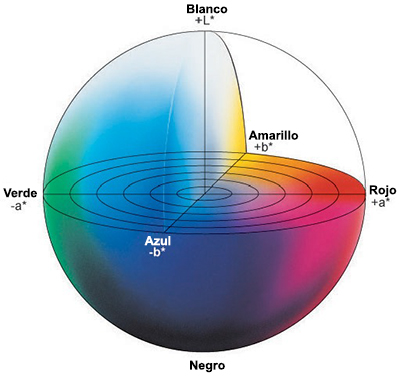
\includegraphics[width=.42\textwidth]{lab1}}
	\subfigure[]{\label{fig:lab-b}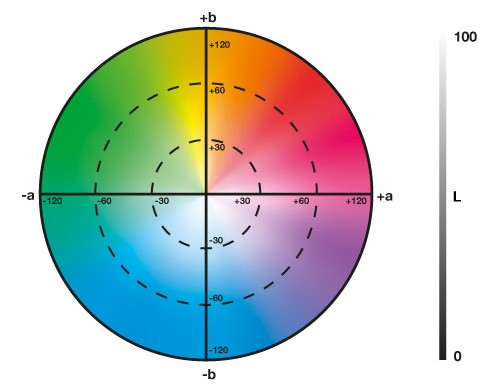
\includegraphics[width=.50\textwidth]{lab2}}
	
	\caption[Espacio de color CIELAB]{Espacio de color CIELAB. En (a) se aprecia el diagrama tridimensional, mientras que en (b) una vista superior del rango de colores con luminancia fija.}
	\label{imagen:lab-color}
\end{figure}

Este es un espacio de color tridimensional descrito por los ejes $a$, que extiende desde verde ($-a$) hasta rojo ($+a$), el eje $b$ que se extiende desde azul ($-b$) hasta amarillo ($+b$), y la luminancia $l$ que varia desde negro ($-l$) hasta blanco ($+l$). Esta representación se puede observar en la figura \ref{imagen:lab-color}.

\subsection{Método de Reinhard}
El objetivo de esta transformación de color es lograr que la distribución de los puntos en el espacio de color LAB se transfieran entre imágenes. Para esto se utiliza la información de la media y desviación estándar sobre cada canal (L, A y B).

Para un par de imágenes $I$ e $I^*$, donde $I$ es la imagen origen e $I^*$ es la imagen que se quiere corregir, se calcula la media y desviación estándar para cada canal.
\begin{align*}
&{\langle l \rangle} \hspace{0.55cm} {\langle l^* \rangle}  &{ \sigma_l } \hspace{0.5cm} { \sigma^*_l } \\
&{\langle a \rangle} \hspace{0.48cm} {\langle a^* \rangle}  &{ \sigma_a } \hspace{0.5cm} { \sigma^*_a }  \\
&{\langle b \rangle} \hspace{0.5cm} {\langle b^* \rangle}  &{ \sigma_b } \hspace{0.5cm} { \sigma^*_b } 
\end{align*}
Luego se ajusta la distribución de la imagen objetivo de la siguiente forma, se le resta la media de la imagen a corregir:
\begin{align*}
l^* &= l^* - \langle l^* \rangle \\
a^* &= a^* - \langle a^* \rangle \\
b^* &= b^* - \langle b^* \rangle
\end{align*}
Luego se escalan los valores en función a las desviaciones estándar:
\begin{align*}
l^* &= \frac{\sigma^*_l}{\sigma_l} l^* \\
a^* &= \frac{\sigma^*_a}{\sigma_a} a^* \\
b^* &= \frac{\sigma^*_b}{\sigma_b} b^*
\end{align*}
Finalmente se le suma la media pero de la imagen origen:
\begin{align*}
l^* &= l^* + \langle l \rangle \\
a^* &= a^* + \langle a \rangle \\
b^* &= b^* + \langle b \rangle
\end{align*}
Para lograr un mapeo de color correcto es necesario obtener la información de desviación estándar y media únicamente en el área de intersección entre las imágenes $I\cap I^*$. De esta forma se logra igualar estas regiones de la imagen que deben corresponder a la misma escena.


\section{Fusión de imágenes}

Una vez se logre determinar la mejor linea de corte, y aplicar una corrección de color, es posible que aun se cuenten con transiciones entre imágenes con cierto nivel de discontinuidad. En este caso es conveniente aplicar algoritmos que permitan una transición suavizada entre dichos bordes.

Se tienen varias versiones de estos algoritmos que serán explicados a continuación: fusión ponderada simple o bajo un esquema piramidal.

\begin{figure}[h]
	\centering     %%% not \center
	\subfigure[]{\label{fig:blend-a}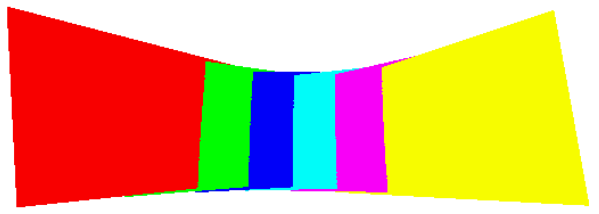
\includegraphics[width=.6\textwidth]{blend-types-1}}
	\vspace{-0.3cm}
	
	\subfigure[]{\label{fig:blend-c}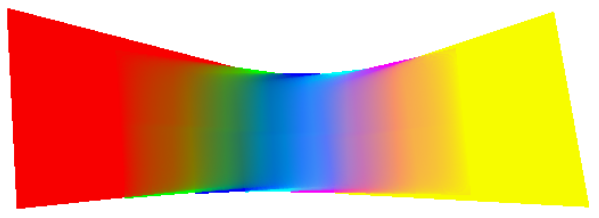
\includegraphics[width=.6\textwidth]{blend-types-3}}
	
	\caption[Tipos básicos de fusión]{Fusión ponderada}
	\label{imagen:blend-types}
\end{figure}

\subsection{Fusión ponderada}
Este tipo de algoritmos realiza una fusión que consiste en realizar un suma ponderada, en la cual se modifica el peso en función de la distancia de los puntos con el borde mas cercano a su imagen. Es decir, se realiza una suma de los valores de las imágenes ($\mathtt{I_1},\, \mathtt{I_2}$) en el área de intersección ($\mathtt{I_1}\cap \mathtt{I_2}$) para cada canal, dándole menor peso a los píxeles que se encuentren mas cercanos del extremo de la imagen. Cabe destacar que esta suma se normaliza para asegurar que no se supere el rango $0-255$ con el cual se representan los valores de la imagen final. La ecuación para la suma ponderada se muestra a continuación:
\begin{displaymath}
	F = \frac{(1-\alpha)\cdot \mathtt{I}_1 + \alpha\cdot \mathtt{I}_2}{512} 
\end{displaymath} 
Donde el parámetro $\alpha$ varia en el rango $0\to 1$, en este caso en función a la distancia, tal y como se ilustra en la figura \ref{imagen:blend-simple}.


\begin{figure}[h]
	\centering
	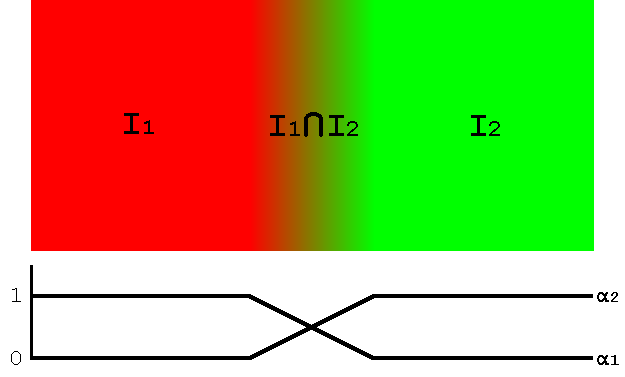
\includegraphics[width=.6\linewidth]{blend1.pdf}
	\caption[Fusión ponderada simple]{Fusión ponderada simple, donde $\alpha_1$ y $\alpha_2$ corresponden con el factor multiplicativo de las imágenes 1 y 2 respectivamente ($\alpha_1 = 1 - \alpha_2$).}
	\label{imagen:blend-simple}
\end{figure}

El algoritmo de fusión ponderada de transición presenta ciertas desventajas, entre estas el efecto fantasma, en el que se observan duplicados de los objetos en la escena pero con cierto grado de desvanecimiento. Si bien no será implementado, el estudio de su funcionamiento es necesario para comprender el algoritmo de fusión que trabaja bajo un esquema piramidal.

\subsection{Fusión ponderada piramidal}



Considerando este problema, y con el objetivo de realizar una unión mas robusta, se desarrolló un esquema piramidal de fusión ponderada. El proceso consiste en obtener una imagen laplaciana para distintos tamaños de escala, formando así una pirámide, al mismo tiempo se va creando para cada nivel de la pirámide una mascara difuminada por el efecto del filtro gaussiano de dicha escala. Luego para cada nivel de la pirámide se aplica el algoritmo de fusión ponderada descrito previamente donde la mascara  difuminada pondera el valor de cada píxel. Entre los trabajos que aplican este algoritmo obteniendo resultados notables se tiene \cite{multiband}, logrando reducir en gran medida el efecto duplicado en las regiones de superposición.

\section{Resultados}

\section{Resumen}


